\documentclass [letter,12pt] {article}
\usepackage{fullpage}
\usepackage{graphicx}
\usepackage[shortlabels]{enumitem}

\title{\huge{\textbf{Music Search++}}}
\author{Jonathan Westerfield \\ \textit{jgwesterfield@tamu.edu}
        \and Matthew Broman \\ \textit{broman334@tamu.edu}}
\date{\today}

\begin{document}

\maketitle

\begin{abstract}
    Spotify uses a music algorithm in order to group songs into music
    playlists. This allows a user to simply choose a song and Spotify will
    choose subsequent songs to play after the current one is finished.
    However, this algorithm is not very effective at choosing songs that are
    similar to the one being played. The algorithm looks at the genre and
    relies on other users groupings and playlists. Often times, the songs
    are not similar but are still in the same genre, which can lead to a
    very jarring transition from a quiet, slow song to a louder, quicker
    one. Examples of this can be Come Sail Away by The Styx transitioning to
    The Grand Illusion by the same band. These two songs are in the same
    genre, the same band, and even in the same album, however, the two songs
    are drastically different in style and volume dynamics.
    
\end{abstract}

\newpage

\section{Objective}
    Our objective is to modify the current Spotify search engine to improve playlist lineups. We will still take into account the genre, artist and album of a song but do some extra analysis to get more information about a song file. We will then create a playlist based off of the song metadata of a single song so that we can create a playlist of songs similar to the one we analyzed.
    
\section{Implementation Breakdown}
    \subsection{Plan}
        \begin{enumerate}
            \item Crawl through Spotify’s songs 
            \item Store the songs
            \item Implement ability to search for songs individually 
                or by artist
            \item Implement ability to create playlist from song that 
                was searched for
        \end{enumerate}
        
    \subsection{Implementation}
        \begin{enumerate}
            \item We got Spotify’s songs using the Spotify API
            \item We stored all of the song information into 
                individual json files
            \item We then uploaded all of our json song files to a 
                Solr Search Engine Instance
            \item We use the Spotify API to search for songs 
        \end{enumerate}
        
\section{Tool Choices}
    \subsection{Solr}
        We chose to use Solr for several reasons. First, it provides robust and efficient text searching.Solr returns search results based on text, making it very easy to implement search functionality based on the numerous parameters in the song data. Solr can perform a search based on any or all fields of a song. In addition, it is very quick and efficient to search based on certain parameters. Another surprising and convenient feature of Solr is the efficient storage of song data. We pulled json data from Spotify that came out to around 1 GB. This was just information and not actually the song audio. However, when we uploaded it to Solr, its final size for our instance only came out to under 15 MB for over 23,000 songs. We created an Amazon AWS EC2 instance (a cloud virtual machine) and installed Solr on it so that it could be accessed quickly and easily over any network. All that is needed to interface with it is the IP address of the server and the query for information. This interface was achieved programmatically using Python connection libraries. An example url string to query Solr is:

        \begin{center}
            \textbf{http://52.14.160.147:8983/solr/SpotifyDB/select?q=artists:``Taylor Swift"}
        \end{center}
        
    \subsection{Spotify API}
        We used the Spotify API for numerous reasons. The most obvious one is that since we are trying to improve the Spotify search algorithm, we might as well use the Spotify API to pull songs so that we can make a fair comparison between our implementation and theirs. The Spotify API provided an easy way to crawl through multiple playlists and pull all of the songs from a single source. In addition, the Spotify API allowed us to pull information about the songs like tempo and energy that was already calculated by Spotify. What specific song data we were able to get from Spotify is in the Song Data section below. In addition, we were able to use the Spotify recommendation feature to pull similar songs. This allowed us to custom tailor our searches for more specific queries. 
        


        
\section{Song Data}
    We stored very detailed song information in order to create more accurate playlists. Every song that went into our data base was stored with its name, artist, album, danceability, liveness, energy, instrumentalness, speechiness, valence, tempo, key, and other information shown below. The song data was uploaded into the Solr Instance in the following format:
    
    \begin{verbatim}
    {
        "album": "Waking Up",
        "artists": "MJ Cole",
        "duration_ms": 224633,
        "episode": false,
        "external_urls": {
            "spotify": "https://open.spotify.com/track/5boGUtIrJjSd2uAueKCHKz"
        },
        "id": "5boGUtIrJjSd2uAueKCHKz",
        "name": "Waking Up",
        "popularity": 36,
        "type": "track",
        "playlists": [
            "37i9dQZF1DX2czWA9hqErK"
        ],
        "key": 11,
        "mode": 0,
        "acousticness": 0.95,
        "danceability": 0.482,
        "energy": 0.211,
        "instrumentalness": 0.0000478,
        "liveness": 0.0929,
        "speechiness": 0.0365,
        "valence": 0.273,
        "tempo": 127.826
    }
    \end{verbatim}
    
\section{Music Search++ CLI}
    We wrote a Python CLI program to facilitate the interface between the user, Solr and Spotify. This CLI lets the user search our Solr database by song name, by artist, or by the songs specific Spotify ID. In addition, the CLI allows the user to create a playlist based on a specific song. The user must input their username, the song ID, the playlist name and the playlist description. The CLI then calls the appropriate functions to get songs similar to the one we specified and create a playlist with those songs. The instructions for the CLI are shown below:
    
    \begin{figure}[htp]
        \centering
        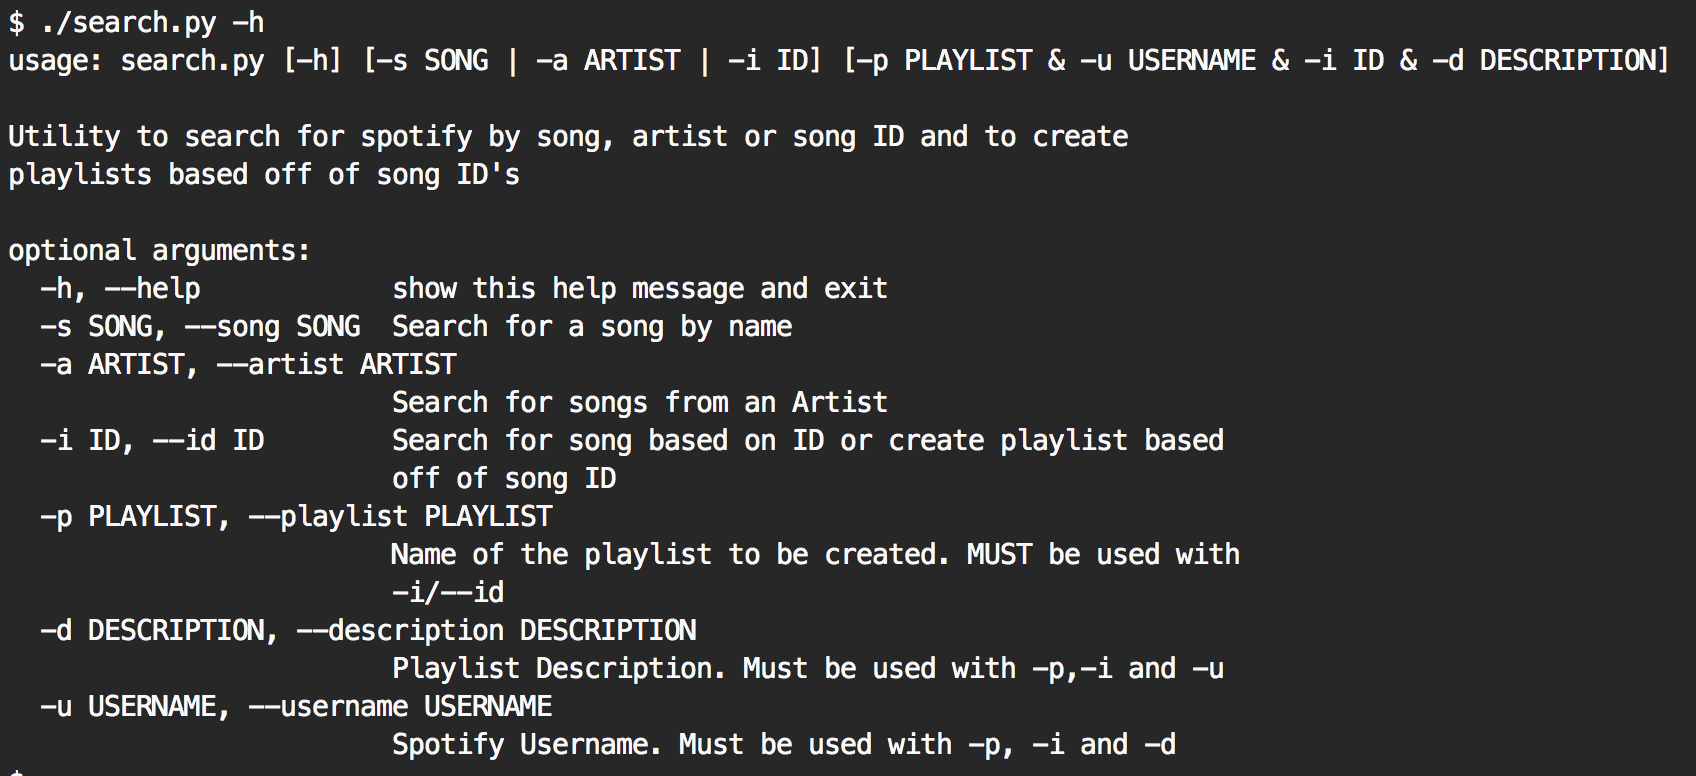
\includegraphics[width=\textwidth]{CLI_Help.png}
        \caption{Music Search++ CLI}
        \label{fig:searchcli}
    \end{figure}

\section{Results}
    \subsection{Song Searching}
        We were able to create playlists using our CLI. This allowed us to achieve fast and accurate song searching either by name of the song or by artist. It returns a result if there is a text match in the results. This means if only a portion of a song name is typed in (maybe the user doens't remember the entire song name) they can still get a list of potential matches. The results of which are shown below:
        
        \begin{figure}[htp]
            \centering
            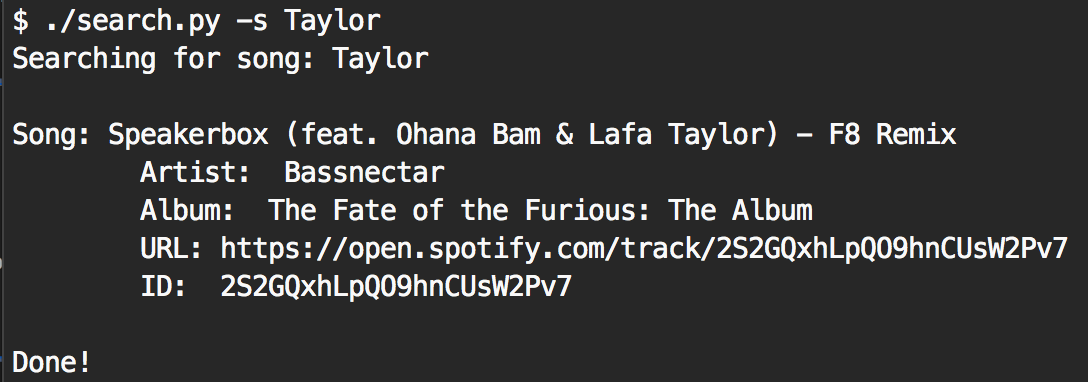
\includegraphics[width=\textwidth]{Song_Taylor_Search.png}
            \caption{Search For Songs Including the Word: ``Taylor"}
            \label{fig:taylorsong}
        \end{figure}
    
        \begin{figure}[htp]
            \centering
            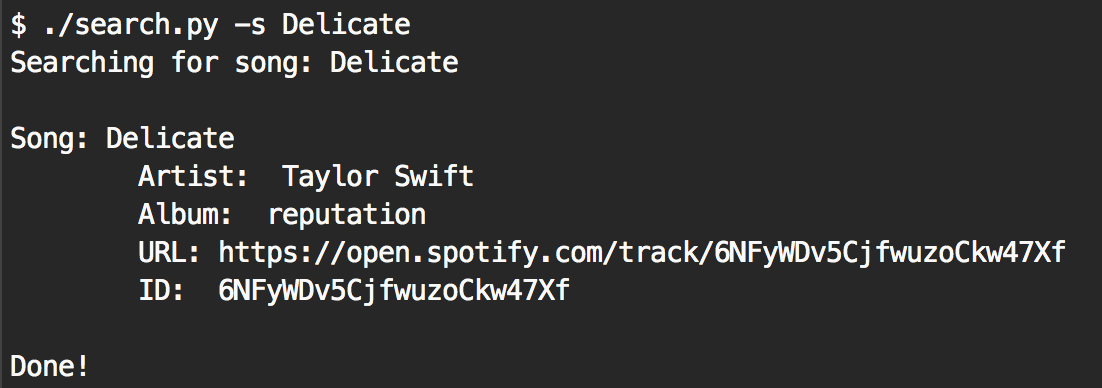
\includegraphics[width=\textwidth]{Delicate_Song_Search.png}
            \caption{Search For the Song: ``Delicate"}
            \label{fig:delicatesong}
        \end{figure}
        
        \begin{figure}[htp]
            \centering
            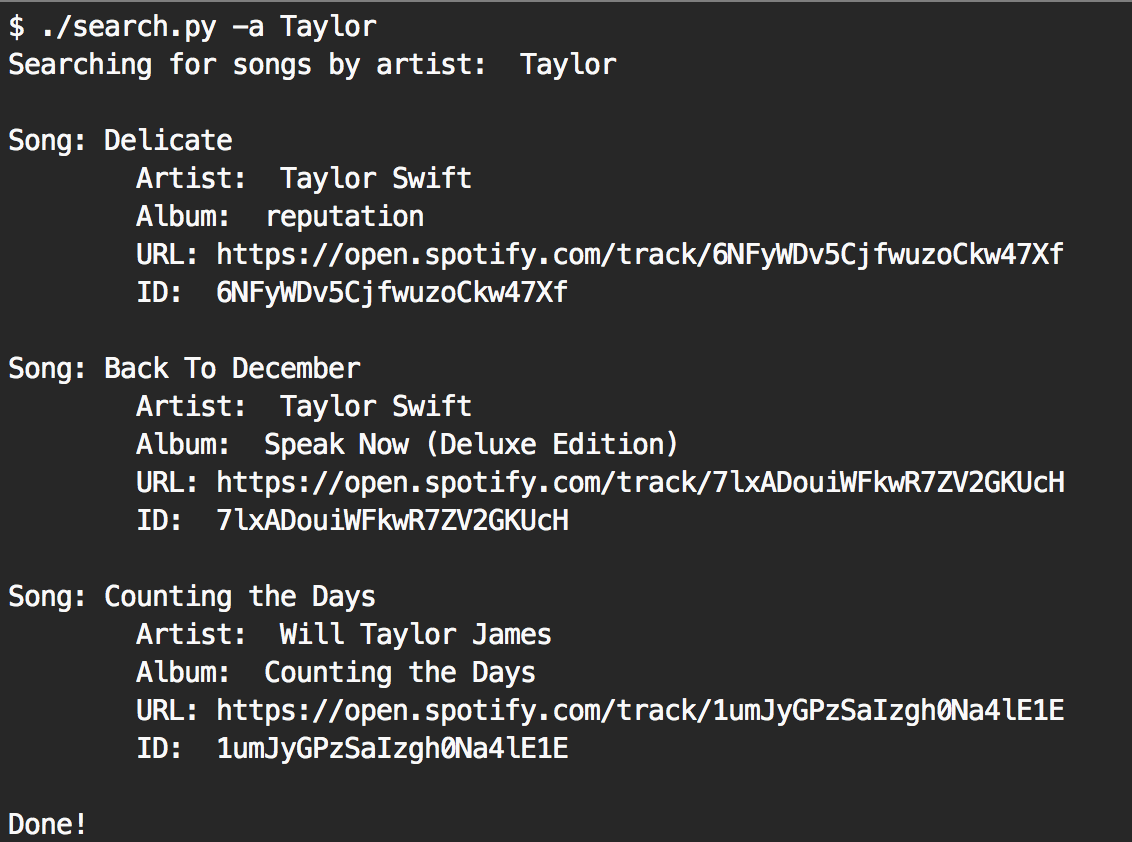
\includegraphics[width=\textwidth]{Artist_Taylor_Search.png}
            \caption{Search For Songs by Artists with ``Taylor"}
            \label{fig:taylorartist}
        \end{figure}
\newpage
    \subsection{Playlist Creation}
        Using our CLI we were able to construct a playlist around a specific song. We search for song ID because it removes any ambiguity or possibility of returning different songs with the same name. We then call the Spotify API, specify the specific metrics with which we want to search for songs, and receive 20 songs back (this number can be increased or decreased). The CLI then creates a playlist using the CLI and populates it with the returned similar songs.
        
        \begin{figure}[htp]
            \centering
            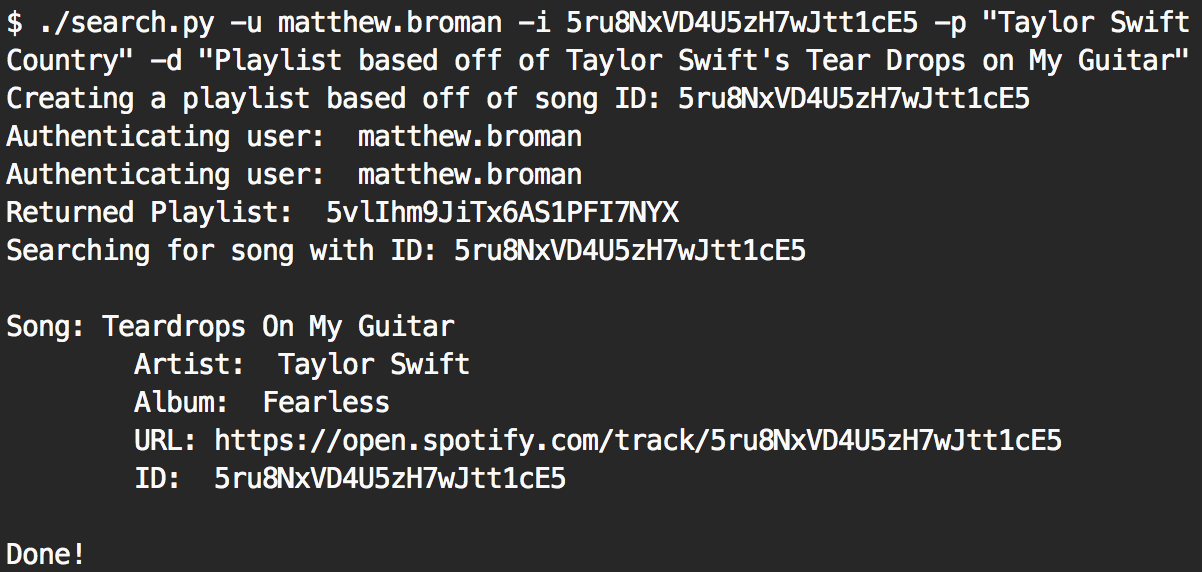
\includegraphics[width=\textwidth]{Playlist_Create.png}
            \caption{Creating a Playlist Based on the Song, ``Teardrop On My Guitar, by Taylor Swift}
            \label{fig:playlistcreate}
        \end{figure}
        
        \begin{figure}[htp]
            \centering
            
\includegraphics[width=\textwidth]{Created_Playlist.png}
            \caption{Playlist Based on the Song, Shoot To Thrill, by AC/DC}
            \label{fig:playlistshoottothrill}
        \end{figure}
        
\newpage
    \subsection{Playlist Analysis}
        We were able to create a playlist based off a single song. In the example above, the playlist was based off of the song Shoot To Thrill by AC/DC. The playlist created had fairly consistent song choice. We actually created a new feature for Spotify. Spotify does not have the option to create a playlist based off a single song. In addition, Spotify usually tries to generate a playlist off of multiple songs, such as recommending songs for adding to a playlist while viewing a specific playlist. In addition, when Spotify recommends songs to be added to a playlist, it usually does so using an amalgamation of song data generated from all of the songs in the playlist. This usually dilutes the song information with information from other songs and can skew the target mood and feel of the returned songs of that search. Also, our returned songs are usually better matches than Spotify's implemenation because we specify ONLY the song metadata as target values to reach. Spotify tries to create a range of song metadata (range of values for liveness, energy, etc.) in order to broaden its search. In addition, we don't include album, artist, or popularity data in the search so this can expand the search to more obscure yet high quality songs that fit our criteria. Due to the characteristics of the song, results are usually in the same genre but are from different artists or the same artist or even in the same album.

        
        
    

    

    
    

\end{document}
